\section{Initial Results}
As mentioned in the previous section, we started by establishing a baseline accuracy by just using the seeding data.
Here are the results from each year and the average overall results.

\vspace{0.5cm}
\begin{tabular}{lc}
  \toprule
  Year & Accuracy\\
  \midrule
  2004 & 0.75\\
  2005 & 0.7187\\
  2006 & 0.6875\\
  2007 & 0.8125\\
  2008 & 0.7656\\
  2009 & 0.75\\
  2010 & 0.6875\\
  2011 & 0.6865\\
  2012 & 0.7313\\
  2013 & 0.7014\\
  2014 & 0.6716\\
  2015 & 0.7910\\
  2016 & 0.7313\\
  2017 & 0.7611\\
  All & 0.7170\\
  \bottomrule
\end{tabular}
\vspace{0.5cm}

So, initially we discovered that the seeding provided a good baseline with a pretty high standard. 
We also saw that the accuracy varies significantly from year to year. 
Furthermore, the potentially noticed that the accuracy has a small negative correlation with the year. 
We should also mention that each year used all the previous years as training data.
This meant that the later years were able to use more data to make their decisions.
In summary, it seems that it is getting harder and harder to predict the outcomes of games based on solely the seed.
Here is a picture of the seeding accuracies for each year in our dataset:

\begin{center}
  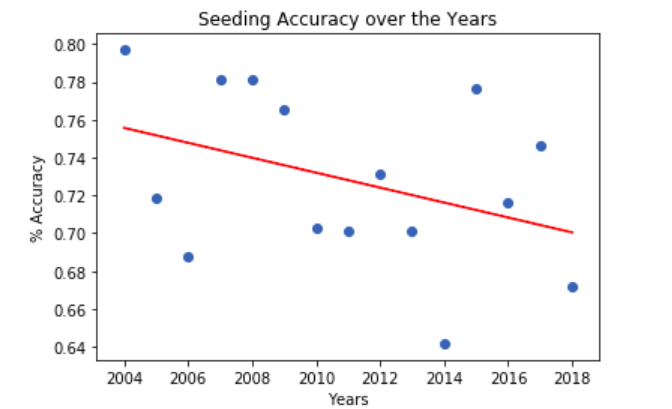
\includegraphics[width=9.5cm]{SeedingAccuracies.png}
\end{center}

Next, we looked at the ability of several top ranking systems to predict the tournament outcomes.
We found that 3 of the ranking systems seemed to outperform the others: RPI, KenPom, and SAG.
Since the seed is technically another ranking system, we included it in this section of data as well.
Here are the results for this set of data as well as how they compare to the baseline.

\vspace{0.5cm}
\begin{tabular}{c c c}
    \toprule
    Year & Accuracy & Difference\\
    \midrule
    2004 & 0.75 & +0.0000\\
    2005 & 0.7343 & +0.0156\\
    2006 & 0.6875 & +0.0000\\
    2007 & 0.8281 & +0.0156\\
    2008 & 0.8281 & +0.0625\\
    2009 & 0.7656 & +0.0156\\
    2010 & 0.6718 & -0.0157\\
    2011 & 0.6865 & +0.0000\\
    2012 & 0.7313 & +0.0000\\
    2013 & 0.6865 & -0.0149\\
    2014 & 0.6865 & +0.0149\\
    2015 & 0.7761 & -0.0149\\
    2016 & 0.7462 & +0.0149\\
    2017 & 0.7611 & +0.0000\\
    All & 0.7193 & +0.0023\\
    \bottomrule
  \end{tabular}
  \vspace{0.5cm}

These initial results helped us establish a baseline accuracy for predicting march madness outcomes.
As we saw in past years and particularly in this year, the tournament prediction is dominated by guessing the correct upsets.
With this in mind, we were interested in trying some new features, making combinations of our features, and enhancing the features that we have.